\documentclass{standalone}
\usepackage{tikz}
\usetikzlibrary{arrows,positioning,calc}
\usepackage{graphicx}
\begin{document}

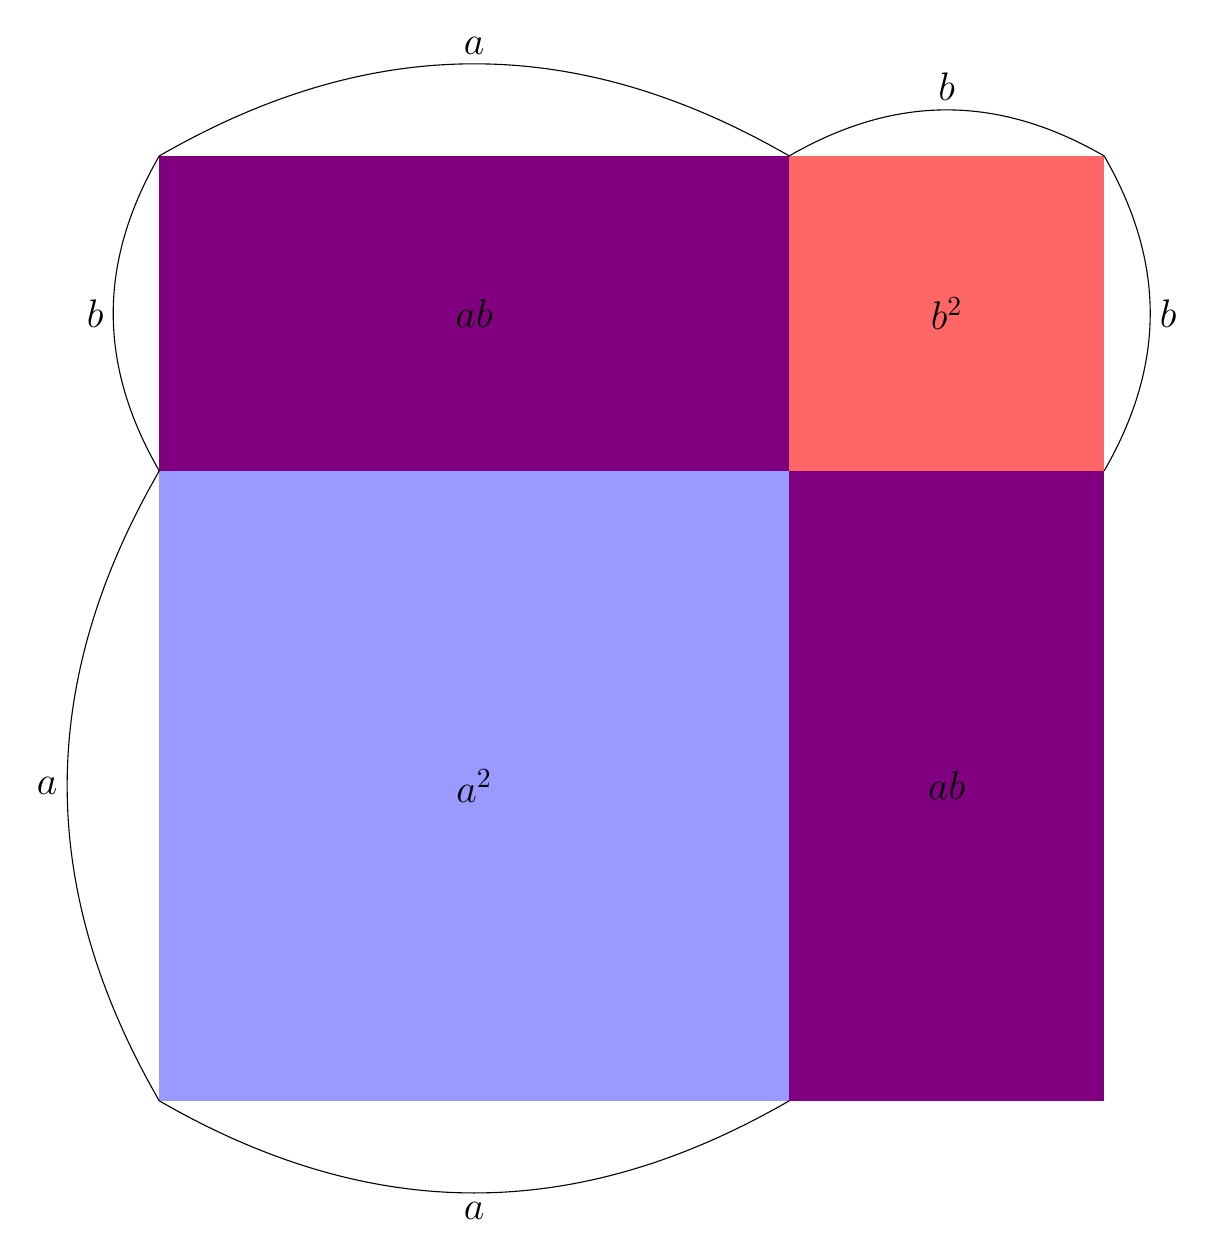
\begin{tikzpicture}[scale = 2.0, font = \Large]
\fill[blue!40!white] (0, 0) rectangle (4, 4);
\fill[red!60!white] (4, 4) rectangle (6, 6);
\fill[red!50!blue] (0, 4) rectangle (4, 6);
\fill[red!50!blue] (4, 4) rectangle (6, 0);
\node at (2, 2) {$a^2$};
\node at (2, 5) {$ab$};
\node at (5, 5) {$b^2$};
\node at (5, 2) {$ab$};
\draw (0, 0) to [bend left] node [midway, left]{$a$} (0, 4) ;
\draw (0, 0) to [bend right] node [midway, below]{$a$} (4, 0);
\draw (0, 4) to [bend left] node [midway, left] {$b$} (0, 6);
\draw (0, 6) to [bend left] node [above] {$a$} (4, 6);
\draw (4, 6) to [bend left] node [above] {$b$} (6, 6);
\draw (6,6) to [bend left] node [right] {$b$} (6, 4);
\end{tikzpicture}
\end{document}